\let\negmedspace\undefined
\let\negthickspace\undefined
\documentclass[journal]{IEEEtran}
\usepackage[a5paper, margin=10mm, onecolumn]{geometry}
\usepackage{lmodern} % Ensure lmodern is loaded for pdflatex
\usepackage{tfrupee} % Include tfrupee package

\setlength{\headheight}{1cm} % Set the height of the header box
\setlength{\headsep}{0mm}     % Set the distance between the header box and the top of the text

\usepackage{gvv-book}
\usepackage{gvv}
\usepackage{cite}
\usepackage{amsmath,amssymb,amsfonts,amsthm}
\usepackage{algorithmic}
\usepackage{graphicx}
\usepackage{textcomp}
\usepackage{xcolor}
\usepackage{txfonts}
\usepackage{listings}
\usepackage{enumitem}
\usepackage{mathtools}
\usepackage{gensymb}
\usepackage{comment}
\usepackage[breaklinks=true]{hyperref}
\usepackage{tkz-euclide} 
\usepackage{listings}
\usepackage{gvv}                                        
\def\inputGnumericTable{}                                 
\usepackage[latin1]{inputenc}                                
\usepackage{color}                                            
\usepackage{array}                                            
\usepackage{longtable}                                       
\usepackage{calc}                                             
\usepackage{multirow}                                         
\usepackage{hhline}                                           
\usepackage{ifthen}                                           
\usepackage{lscape}
\begin{document}

\bibliographystyle{IEEEtran}
\vspace{3cm}

\title{1-1.8-2}
\author{EE24BTECH11005 - Arjun Pavanje
}
% \maketitle
% \newpage
% \bigskip
{\let\newpage\relax\maketitle}
Question:\\
Find the distance between the following pairs of points\\
\begin{enumerate}
	\item $(2,3,5)$ and $(4,3,1)$
	\item $(-3,7,2)$ and $(2,4,-1)$
	\item $(-1,3,-4)$ and $(1,-3,4)$
	\item $(2,-1,3)$ and $(-2,1,3)$
\end{enumerate}
\solution
\begin{table}[h!]    
  \centering
  \begin{tabular}[12pt]{ |c| c|}
    \hline
    \textbf{Variable} & \textbf{Description}\\ 
    \hline
	$\vec{a}$ & $BC$ line\\
   \hline
	$\vec{b}$ & $AC$ line\\
   \hline
	$\vec{c}$ & $AB$ line, $5cm$ length\\
   \hline
	$\vec{K}$ & $a+b=5cm$\\
	\hline
	$\vec{\angle{A}}$ & $\angle{BAC}=45{\degree}$\\
	\hline

    \end{tabular}

  \caption{Variables Used}
  \label{tab1-1.5-29}
\end{table}\\
\begin{enumerate}
\item 
\begin{align}
	a_2-a_1 &= \myvec{
		2\\
		0\\
		-4\\
	}\\
	\norm{a_2-a_1} &= \sqrt{(a_2-a_1)^T (a_2-a_1)} = \sqrt{20}
\end{align}\\
Distance = $\sqrt{20}$
\item 
\begin{align}
	b_2-b_1 &= \myvec{
		5\\
		-3\\
		-3\\
	}\\
	\norm{b_2-b_1} &= \sqrt{(b_2-b_1)^T (b_2-b_1)} = \sqrt{43}
\end{align}\\
Distance = $\sqrt{43}$

\item 
\begin{align}
	c_2-c_1 &= \myvec{
		2\\
		-6\\
		8\\
	}\\
	\norm{c_2-c_1} &= \sqrt{c_2-c_1)^T (c_2-c_1)} = \sqrt{104}
\end{align}\\
Distance = $\sqrt{104}$
\item 
\begin{align}
	d_2-d_1 &= \myvec{
		-4\\
		2\\
		0\\
	}\\
	\norm{d_2-d_1} &= \sqrt{(d_2-d_1)^T (d_2-d_1)} = \sqrt{20}
\end{align}\\
Distance = $\sqrt{20}$
\end{enumerate}
\begin{figure}[h!]
   \centering
   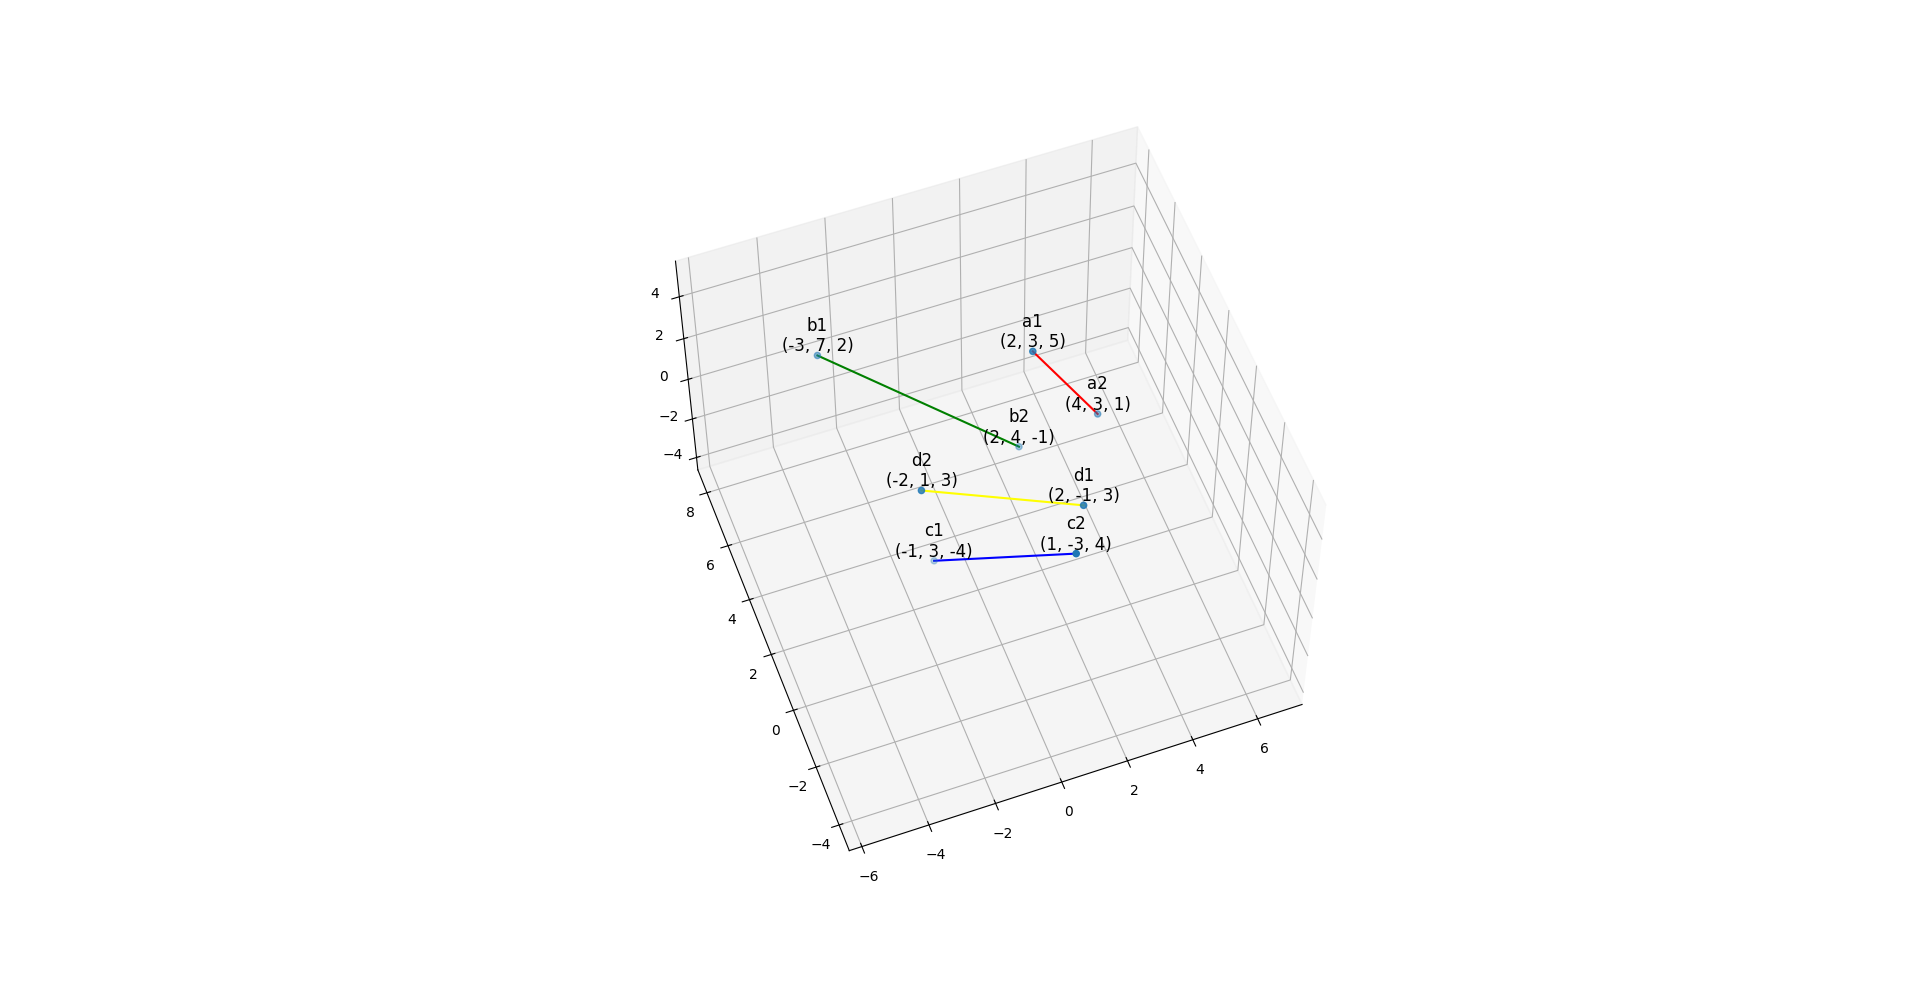
\includegraphics[width=0.7\linewidth]{figs/Figure_1.png}
   \caption{Plot of the points}
   \label{stemplot}
\end{figure}
\end{document}
